\documentclass{beamer}
\usepackage[utf8]{inputenc}
\usepackage[T1]{fontenc}

\usebackgroundtemplate{
	
\includegraphics[width=\paperwidth,height=\paperheight]{img/background}
}

\title{Chapter 01: Structured Analysis}

\author[P.A. Nugroho]{Pascal Alfadian Nugroho}
\institute[IF-UNPAR]{Program Studi Informatika, \\Universitas Katolik Parahyangan}

\begin{document}
	\begin{frame}
		\titlepage
	\end{frame}
	
	\section{Specification Document}
	\subsection{Overview}
	\begin{frame}{Specification Document}
		\begin{itemize}
			\item Contract between client and developer
			\item Specifies precisely what the product must do and constraints of the product
			\item Almost always, includes deadline
			\item Includes set of acceptance criteria
			\item \textbf{Does not} specify how the product is made unless specifically needed
			\item There can be many ways in writing a specification document
		\end{itemize}
	\end{frame}
	\subsection{Example}
	\begin{frame}{Specification Document: Example}
		\begin{center}
			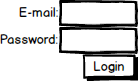
\includegraphics[scale=0.5]{img/01_login}
		\end{center}
		\begin{enumerate}
			\item The login screen must show two inputs: email and password
			\item Password must be transmitted securely to server using HTTPS
			\item The error message for ``unregistered user'' and ``invalid password`` must be exactly the same
			\item \textit{The login screen must be implemented using HTML5 and CSS3 standard} % example of requirement that specifically governs how the product is made
		\end{enumerate}
	\end{frame}
	\subsection{Goals}
	\begin{frame}{Specification Document: Goals}
		\begin{itemize}
			\item Agreement between client/user and development team
			\item Let development team fully understands the problem
			\item Hence a \textit{solution strategy}(-ies) can be suggested
		\end{itemize}
	\end{frame}

	\section{Informal Specifications}
	\subsection{Overview}
	\begin{frame}{Informal Specifications}
		Example of informal specification using \textit{natural language} \cite[page 462]{Schach:2006:OCS:1207045}:
		\begin{quotation}
		BV.4.2.5. If the sales for the current month are below the target sales, then a report is to be printed, unless the difference between target sales and actual sales is less than half of the difference between target sales and actual sales in the previous month or if the difference between target sales and actual sales for the current month is under 5 percent.
	\end{quotation}
	\end{frame}
	\subsection{Problems}
	\begin{frame}{Informal Specifications: Problems}
		\begin{itemize}
			\item Lengthy sentence to explain accurately what the product should behave
			\item Ambiguous, e.g. when comparing to last month, is it in terms of percentage or in dollars?
		\end{itemize}
	\end{frame}	
	
	\section{References}
	\begin{frame}[allowframebreaks]
	        \frametitle{References}
	        \bibliographystyle{amsalpha}
	        \bibliography{module_01}
	\end{frame}
\end{document}

